% =====================================================================
% 第 2 节  二维 CFT 的定义性质（原书 p.1–p.4 上半）
% 对应图像 work/pages/page_001.png – page_004.png
% =====================================================================

\section{二维 CFT 的定义性质}\label{sec:2}

\begin{keytakeaways}
  \item \textbf{物理图像}：二维幺正 CFT = 局域算符的希尔伯特空间 + 态-算符对应 + 无迹能动张量。柱面上的态与平面上的局域算符一一对应，能动张量在 OPE 中生成 Virasoro 代数。
  \item \textbf{数学工具}：径向量子化、Laurent 展开、Ward 恒等式、Schwarzian 导数、指数映射（平面 $\leftrightarrow$ 柱面）。
  \item \textbf{本节结论}：算符乘积展开（OPE）的结合性（等价于球面四点函数的交叉对称性）加上原初算符环面单点函数的模协变性，构成二维 CFT 的全部自洽性条件。
\end{keytakeaways}

一个二维幺正 CFT 拥有由局域算符构成的希尔伯特空间 $\mathcal{H}$；由态-算符对应，它与柱面 $\mathbb{R}\times S^1$ 上 CFT 态空间的希尔伯特空间典范同构。眼下我们假定 CFT 是\emph{紧致的}，即算符谱离散，特别地包含单位算符 $\mathbf{1}$；后者对应柱面上可归一化的基态 $|0\rangle$。稍后我们会考虑非紧致 CFT 的例子，届时这一性质将适当放宽。

此外，二维 CFT 具有守恒的无迹能动张量 $T_{\mu\nu}$。无迹条件 $T^{\mu}_{\ \mu}=0$ 等价于共形不变性；在平直二维时空中它以算符等式成立。在弯曲时空中，由于共形反常，这一条件被替换为
\begin{equation*}
  T^{\mu}_{\ \mu} = -\frac{c}{12}R,
\end{equation*}
其中 $c$ 是 CFT 的中心荷，$R$ 是二维时空的 Ricci 标量。\footnote{当然，这种情况下也可以坚持只谈论 $T_{\mu\nu}$ 的无迹部分，但那样的算符不再守恒。}

% [Tutor Note: 共形反常的系数与符号依赖约定：原文取使 (2.1) 中 $c/(2z^4)$ 与 (2.9) 中 $+c/24$ 同时成立的归一化。不同教材可能把 $T^\mu_{\ \mu}$ 写成 $+\frac{c}{12}R$，差别只在 $R$ 或 $T_{\mu\nu}$ 的符号定义，不影响物理。]

\begin{figure}[htbp]
  \centering
  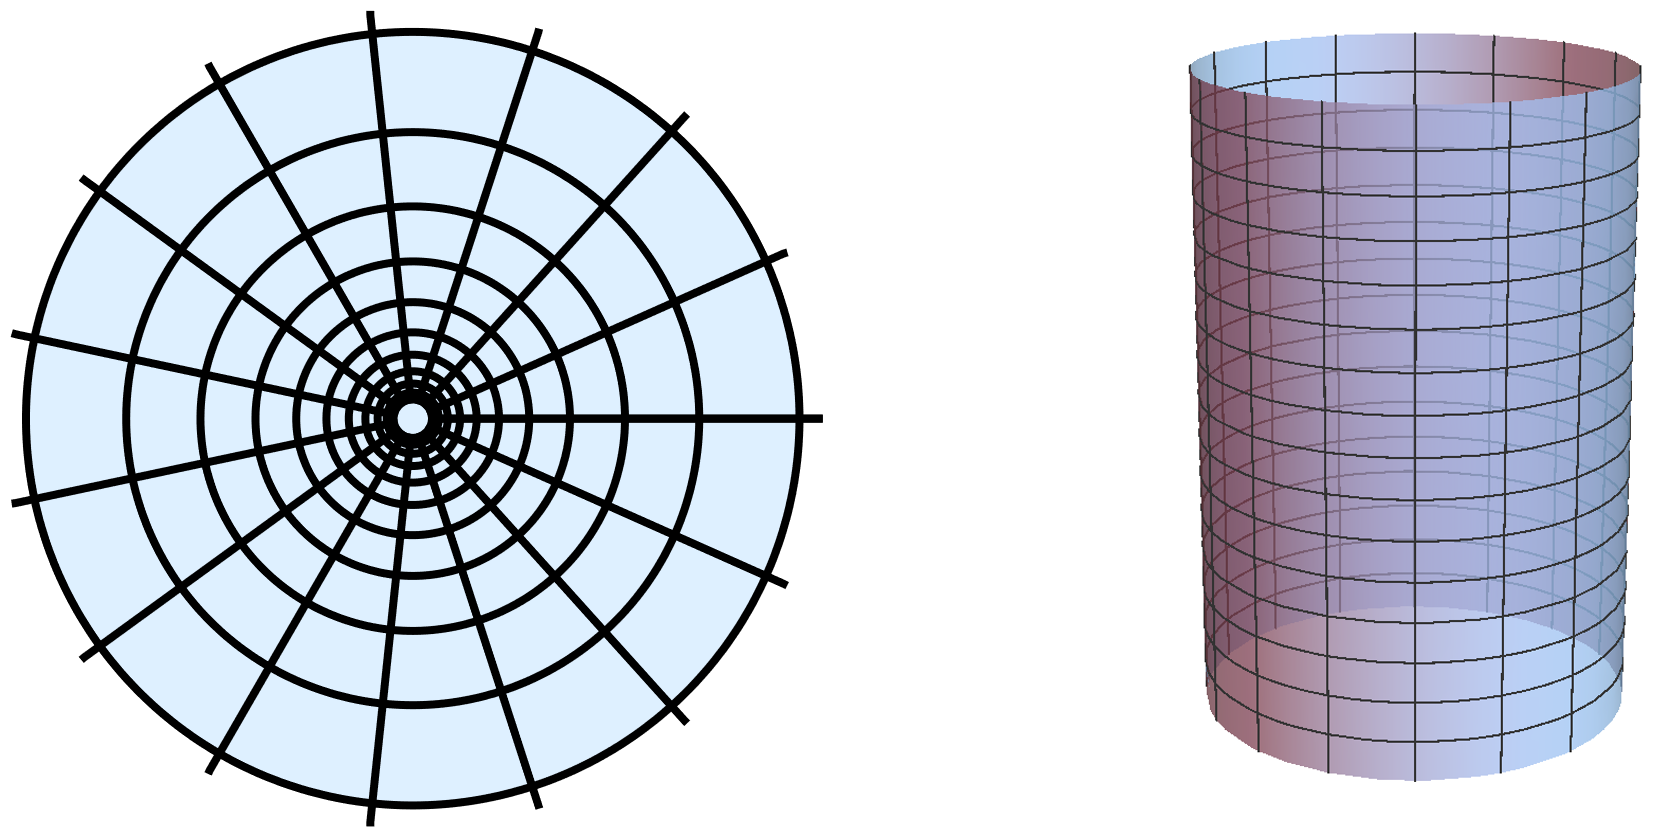
\includegraphics[width=0.72\textwidth]{figures/fig01.png}
  \caption{平面原点处的局域算符，在态-算符对应下映射为圆/柱面上 CFT 的一个态。（原文 p.2，图 1）}
  \label{fig:1}
\end{figure}

在算符乘积展开下，能动张量生成 Virasoro 代数。局域算符空间 $\mathcal{H}$ 构成 Virasoro 代数的一个表示，它可分解为不可约表示的直和，每个不可约表示都含有一个最低维的"原初"算符。

\begin{figure}[htbp]
  \centering
  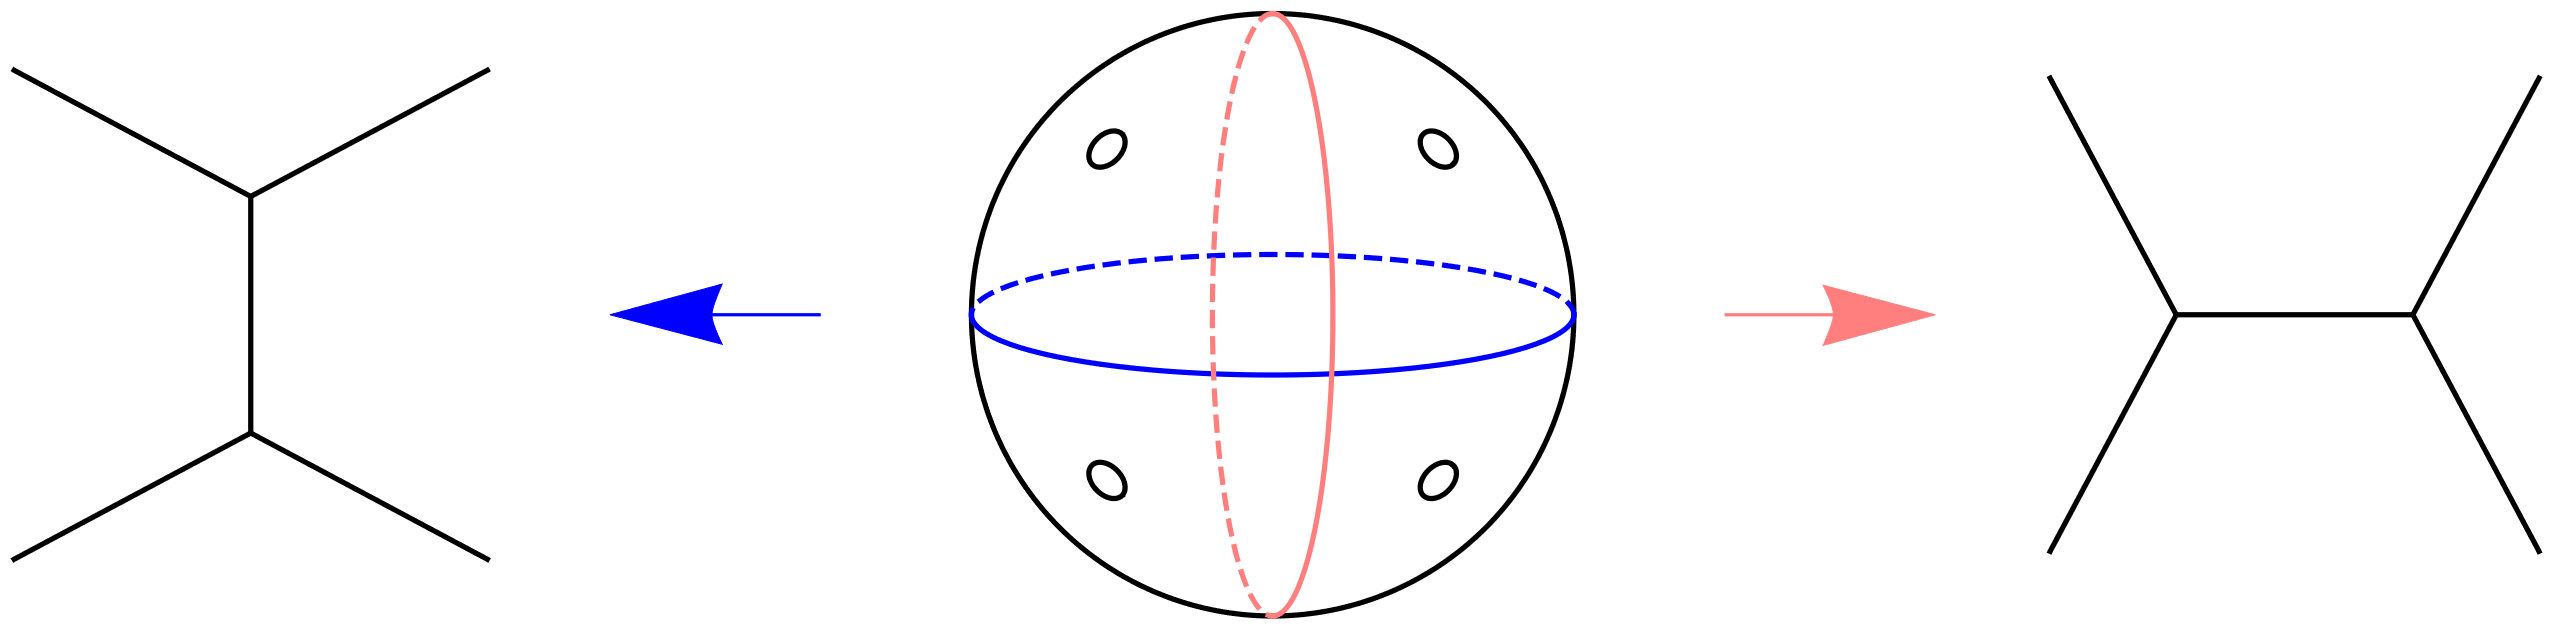
\includegraphics[width=0.92\textwidth]{figures/fig02.png}
  \caption{OPE 的结合性等价于球面四点函数的交叉对称性。（原文 p.2，图 2）}
  \label{fig:2}
\end{figure}

\begin{figure}[htbp]
  \centering
  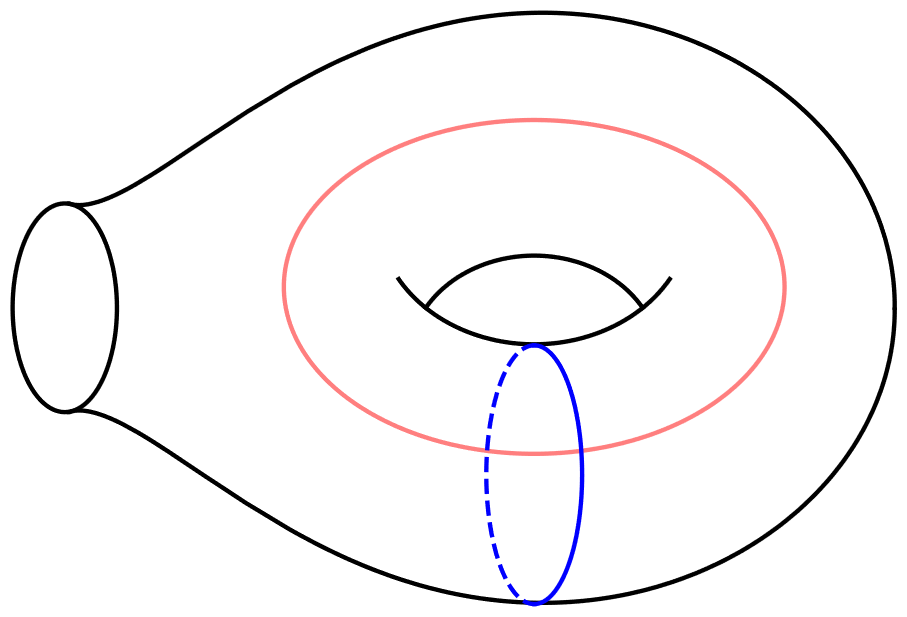
\includegraphics[width=0.40\textwidth]{figures/fig03.png}
  \caption{环面单点函数的模协变性是二维 CFT 的另一条关键自洽性条件。（原文 p.2，图 3）}
  \label{fig:3}
\end{figure}

平面上（或共形等价的黎曼球面上）分离点处的局域算符关联函数有良好定义，且完全由算符乘积展开确定。利用局域算符作为圆周上态的完备性，通过管道化（plumbing）构造，可以在任意黎曼面上构造局域算符的关联函数。二维 CFT 在一般黎曼面上的自洽性要求：由不同"裤子"分解的管道化构造算出的关联函数必须彼此一致。这实际上等价于 OPE 的结合性（球面四点函数的交叉不变性），再加上原初算符环面单点函数的模协变性 \cite{r1}。

\subsection{Virasoro 代数}\label{subsec:2.1}

在欧氏平面上，取复坐标 $(z,\bar z)$，线元为 $\dd s^2=\dd z\,\dd\bar z$。能动张量有两个独立分量：$T(z)\equiv T_{zz}(z)$ 与 $\bar T(\bar z)\equiv T_{\bar z\bar z}(\bar z)$。一对能动张量（比如全纯分量）的 OPE 为
\begin{equation}
  \label{eq:2-1}
  T(z)T(0) \sim \frac{c}{2z^4} + \frac{2}{z^2}T(0) + \frac{1}{z}\partial T(0),
\end{equation}
其中已略去 $z\to0$ 极限下的非奇异项。右端 $z^{-2}$ 阶项由膨胀对称性（其 Noether 流为 $zT(z)$）对应的 Ward 恒等式决定，$z^{-1}$ 阶项则由平移对称性（由 $T(z)$ 生成）对应的 Ward 恒等式决定。假定不存在负维数算符，且唯一的零维算符正比于单位算符，则 (2.1) 就是 $TT$ OPE 最一般的形式（注意 $z^{-3}$ 项会与 OPE 的交换性冲突）。

% [Tutor Note: (2.1) 的三个系数不是独立的：$z^{-4}$ 系数是中心荷 $c/2$，$z^{-2}$ 系数恒为 2，$z^{-1}$ 系数恒为 1，后两者由 $T$ 的维数（2）与 Ward 恒等式固定，不能随意改动。这几个数字是后面所有共形块计算的基准，抄写时极易漏掉因子 2。]

在原点处存在局域算符 $\mathcal{O}(0)$ 时，$T(z)$ 在 $\mathbb{C}\backslash\{0\}$ 上全纯。于是 $T(z)$ 有 Laurent 级数表示
\begin{equation}
  \label{eq:2-2}
  T(z)=\sum_{n=-\infty}^{\infty}\frac{L_n}{z^{n+2}},
  \qquad
  L_n=\oint\frac{\dd z}{2\pi i}\,z^{n+1}T(z),
\end{equation}
该级数在以原点为中心、内部不再插入其他局域算符的圆环上收敛（在关联函数的意义下）。类似地，定义 $\bar L_n$ 为 $\bar T(\bar z)$ 的反全纯 Laurent 系数。$L_n$ 生成中心荷为 $c$ 的 Virasoro 代数
\begin{equation}
  \label{eq:2-3}
  [L_n,L_m]=(n-m)L_{n+m}+\frac{c}{12}(n^3-n)\,\delta_{n,-m},
\end{equation}
同样 $\bar L_n$ 生成另一份 Virasoro 代数，其中心荷 $\tilde c$ 可以不同。

% [Tutor Note: $L_n$ 的定义式 (2.2) 中幂次是 $z^{n+1}$，相应地 $T(z)=\sum L_n z^{-n-2}$；若换成 $z^{-n-2}$ 的另一种约定，对易关系 (2.3) 的 $c$ 项不变但 $n$ 的移位会变。核对后续共形块公式时务必以此处幂次为准。]

一般的无穷小共形变换由 Noether 流
\begin{equation}
  \label{eq:2-4}
  (j_z,j_{\bar z})=\bigl(-\epsilon(z)T(z),\,-\tilde\epsilon(\bar z)\bar T(\bar z)\bigr)
\end{equation}
生成。局域算符 $\mathcal{O}(z,\bar z)$ 的相应变换为
\begin{equation}
  \label{eq:2-5}
  \delta_\epsilon\mathcal{O}(z,\bar z)
  =-\oint_{C_z}\frac{\dd w}{2\pi i}\,\epsilon(w)T(w)\mathcal{O}(z,\bar z)
  +\oint_{C_z}\frac{\dd\bar w}{2\pi i}\,\tilde\epsilon(\bar w)\bar T(\bar w)\mathcal{O}(z,\bar z),
\end{equation}
其中 $C_z$ 是逆时针环绕 $z$ 的围道。特别地，由此可推出能动张量 $T(z)$ 自身的无穷小共形变换：
\begin{equation}
  \label{eq:2-6}
  \delta_\epsilon T(z)=-\frac{c}{12}\partial^3\epsilon(z)-2\partial\epsilon(z)T(z)-\epsilon(z)\partial T(z).
\end{equation}

% [Tutor Note: (2.5) 的围道积分把算符的变换写成"把 $\epsilon T$ 与算符做径向序乘积再取留数"，这正是径向量子化下 Ward 恒等式的标准形式；第二个积分中 $\bar w$ 围道的取向与全纯部分相反，两部分的相对符号是初学者最容易出错的地方。]

把无穷小变换复合起来便得到有限共形变换。用与之相伴的全纯微分同胚来刻画较为方便，其无穷小形式为
\begin{equation}
  \label{eq:2-7}
  z\mapsto z'(z)=z+\epsilon(z).
\end{equation}
过渡到由 $z'=f(z)$ 表示的有限共形变换，$T(z)$ 变换为 $T'(z)$，满足
\begin{equation}
  \label{eq:2-8}
  \left(\frac{\partial z'}{\partial z}\right)^{2}T'(z')=T(z)-\frac{c}{12}\{z',z\},
\end{equation}
其中
$\displaystyle \{z',z\}=\frac{2\partial^3 z'\,\partial z'-3(\partial^2 z')^2}{2(\partial z')^2}$
是 Schwarzian 导数。

% [Tutor Note: Schwarzian 导数的定义各书相差一个整体符号与因子 2；检验约定是否一致的最快办法是取 $z'=z+\epsilon$，(2.8) 应回到 (2.6)。另外 $\{z',z\}$ 对 Möbius 变换 $z'=(az+b)/(cz+d)$ 恒为零，这正是全局共形变换下 $T$ 按张量变换的原因。]

共形变换的一个基本而重要的例子，是从以 $w$ 参数化的欧氏柱面到以 $z$ 参数化的复平面的指数映射 $z=e^{-iw}$：
\begin{equation}
  \label{eq:2-9}
  T_{ww}(w)=(\partial_w z)^2T_{zz}(z)+\frac{c}{24}.
\end{equation}
原点处有算符时 $T_{zz}(z)$ 的 Laurent 展开，此时变为柱面上 $T_{ww}(w)$ 的 Fourier 展开：
\begin{equation}
  \label{eq:2-10}
  T_{ww}(w)=-\sum_{n=-\infty}^{\infty}L_n\,e^{inw}+\frac{c}{24}.
\end{equation}
类似地有
\begin{equation}
  \label{eq:2-11}
  \bar T_{\bar w\bar w}(\bar w)=-\sum_{n=-\infty}^{\infty}\bar L_n\,e^{-in\bar w}+\frac{\tilde c}{24}.
\end{equation}

% [Tutor Note: (2.9) 与 (2.10) 中的常数 $+c/24$ 是柱面上的 Casimir 能，来自 $z=e^{-iw}$ 的 Schwarzian 导数：$\{e^{-iw},w\}$ 给出 $1/2$，乘 $-c/12$ 并补上 $( \partial_w z)^2$ 的贡献后正好是 $c/24$。从 (2.9) 到 (2.10) 只需代入 $z^{-n-2}=e^{i(n+2)w}$ 与 $(\partial_w z)^2=-e^{-2iw}$，读者应亲手验证一次符号。]

记 $w=\sigma+i\tau$，取 $\tau=-it$ 即可解析延拓到洛伦兹号差。如此 $w=\sigma+t$ 与 $\bar w=\sigma-t$ 成为两个独立的实参数。此外，在洛伦兹号差下能动张量分量 $T_{ww}$ 与 $\bar T_{\bar w\bar w}$ 是厄米算符。于是算符 $L_n$ 的厄米共轭为 $L_{-n}$，同样 $\bar L_n^{\dagger}=\bar L_{-n}$。按定义，幺正 CFT 在（洛伦兹）柱面上的态构成全纯与反全纯 Virasoro 代数的幺正表示。
